% !TEX encoding = UTF-8 Unicode
% !TEX TS-program = XeLaTex

\documentclass[
	a0,
	portrait
	]{a0poster}

\usepackage{multicol}
\columnsep=60pt 
\columnseprule=1pt
\def\columnseprulecolor{\color{cbordeaux}}

\usepackage[svgnames]{xcolor} 

\usepackage{palatino} 

\usepackage{lipsum}

\usepackage{graphicx} % Required for including images
\graphicspath{{img/}} % Location of the graphics files

\usepackage{booktabs} % Top and bottom rules for table
\usepackage[
	font=small,
	labelfont=bf
	]{caption} % Required for specifying captions to tables and figures

\usepackage{
	amsfonts,
	amsmath,
	amsthm,
	amssymb
	} % For math fonts, symbols and environments
	
\usepackage{wrapfig} % Allows wrapping text around tables and figures

\usepackage{tikz}
\usetikzlibrary{
	shapes,
	arrows
	}

\usepackage{float}

\usepackage{color}

\usepackage{
	fontspec,
	xltxtra,
	xunicode
	}

\usepackage[italian]{babel}
	
\defaultfontfeatures{Mapping=tex-text}

\setromanfont[Mapping=tex-text]{Fira Sans}

\setsansfont[
	Scale=MatchLowercase,
	Mapping=tex-text
	]{Fira Sans}
	
\setmonofont[]{Fira Mono}

\definecolor{cpurple}{RGB}{39, 79, 134} % #514594
\definecolor{cbordeaux}{RGB}{133, 39, 78} % #993366

\usepackage{multirow}

\usepackage{booktabs}

\usepackage{tabularx}

\usepackage{titlesec}

\usepackage{lettrine}

\titlespacing*{\section}{0pt}{0\baselineskip}{0.1\baselineskip}
\titlespacing*{\subsection}{0pt}{0\baselineskip}{0.5\baselineskip}

\renewcommand\footnoterule{}

\usepackage{hyperref}
\usepackage{cleveref}

\crefformat{footnote}{#2\footnotemark[#1]#3}

% ------------------------------------ DOCUMENT
  
\begin{document}

\color{cpurple} 

% ------------------------------------ TESTATA

\begin{table}[htp]
\color{cpurple} 
\begin{center}
\begin{tabularx}{\textwidth}{Xc}
\veryHuge \textbf{\color{cbordeaux}SEAM} & \multirow{ 5}{*}{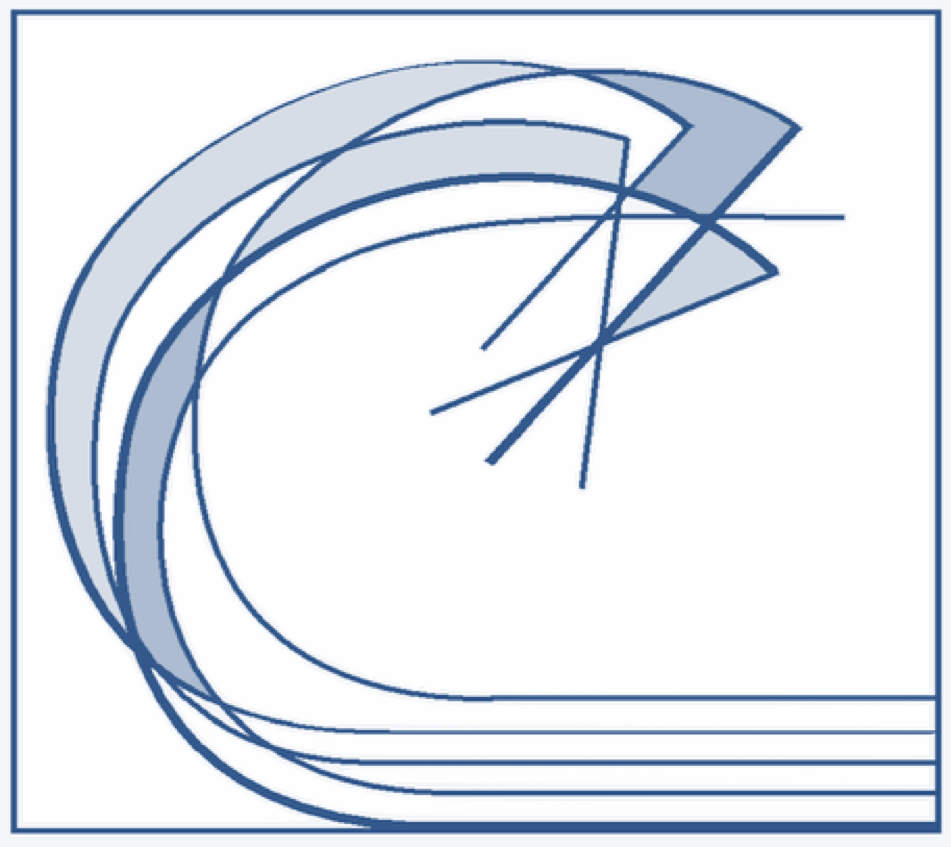
\includegraphics[scale=.35]{274f86logo}} \\
\Huge \textit{Sustained Electro-Acoustic Music} & \\[1.cm]
\huge \textbf{\color{cbordeaux}Giuseppe Silvi, Davide Tedesco} & \\[0.2cm]
\huge Conservatorio S. Cecilia di Roma & \\[0.2cm]
\Large \texttt{s-e-a-m.github.io} & \\[1.2cm]
\large \textit{Research report:} & CONSERVATORIO S. CECILIA DI ROMA \\[0.2cm]
\huge  \textbf{\color{cbordeaux}I am sitting in a room • Risonanze Erranti • Mobile Locale} &  \\ 
\end{tabularx}
\end{center}
\label{default}
\end{table}%   

\large

% ------------------------------------ ABSTRACT

\noindent \emph{Sustained Electro-Acoustic Music} is a project inspired by Alvise Vidolin and Nicola Bernardini's article \cite{bevi05} on \emph{live electroacoustic music sustainability}. In their text, they point at multiple technical faces of the sustainability problem such as technological, notational or general conception issues. Even if the article aforementioned focuses only on \emph{live} electroacoustic music, the concept of sustainability is applicable to any kind of documented music that uses electroacoustic environments including therefore the acousmatic works, instruments mixed with tape and structured amplified works. This will be the purpose of the presented text. • 
The ambition of this project is to grow the interpretation and the electroacoustic musical practice with the consciousness of the electronic and informatics problems that had made arduous to approach this music and prevented the growth of interpretative thinking. It is possible, with a community structure, to determine, build and stratify interpretation of musical core, the repertoire, concealing the environment-related technological issues. They are instruments, not the music itself, after all.
When we refer to a virtuoso musician, we often point at a violinist or at a piano player: someone who intensely practice on his instrument. This is the central point: Does the violinist builds its own violin every time he approaches a new composition? Does the pianist? The electroacoustic musician does it, every time.
Referring to the electroacoustic music literature, where the substantial difference with the acoustical one is an inevitable continuously changing of the environment, we prefer to use the topology classification in place of typology one. A typology classification is, according to general type, used where characteristics of something are fixed and produce a catalogue of things. A topology classification considers instead the time-space characteristics of shape and permits the time variance of the environments. We classify three topologies of the electroacoustic music in literature:

\begin{description}
  \item[The undocumented] where composers use only word description to generate environment and circumstances;
  \item[The \emph{words-hole}] where the score has deep technical documentation but listing names of undocumented instruments. Without musicological methodologies, frequently with names without a specific meaning;
  \item[The porting] where informatics translations between languages or informatics technologies are based on literature and shared knowledge.
\end{description}

The identification of topological classes in place of typological forms is necessary to subordinate technology-matter to the musical practice and poetics.

\normalsize

% ------------------------------------ CORPO

\begin{multicols}{4}

\begin{center}
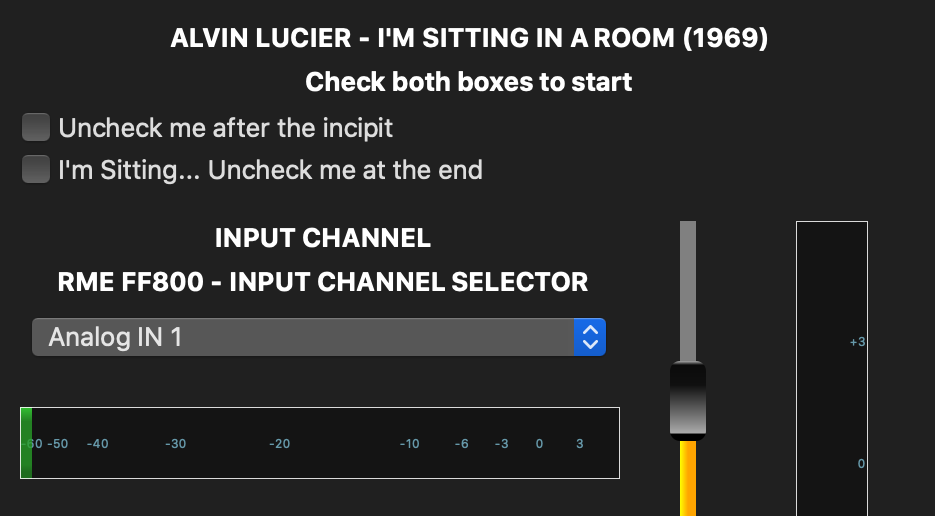
\includegraphics[width=1.\linewidth]{lais-GUI}
\end{center}

% ------------------------------------ ELENA

\section*{\color{cbordeaux}WRITING \\THE UNDOCUMENTED}

\emph{The undocumented} topology holds all works in which composers used only word descriptions to portray the electroacoustic performing environment, with the rules and circumstances needed. There are tons of scores that implicitly involves particular amplification, or complex electroacoustic staging, only by words description. 


Speaking at beginner music students about Lucier's \emph{\textbf{I am sitting in a room}}, is a kind of sharing of a multilevel experience. There are a lot of access layers each with different bits of knowledge requirements. One of these, of course, is how you can do it today. 

The score state a text to be read, it explains what is going to happen and why, so the process unveils the process itself. The acoustical properties of the space transform the speech. The “resonant frequency of the room reinforces themselves”, while the others are absorbed, they are attenuated by space. Space as an instrument to be played and articulated by time. 

The very deep sustainability problem of that work isn't technical. It is a simple process. The very deepest problem is sensibility. The worst thing that can happen to the \emph{process-music} is the perfect process execution without the music. To seam process and music we need to unfold ears and minds to the Lucier's perception and sensibility. 

How? Doing it, like he exactly suggested fifty years ago: practising. 

\vfill

\begin{quotation}
\begin{it}
\begin{flushright}
\noindent Make versions in which one recorded statement is recycled through many rooms. Make versions using one or more speakers of different languages in different rooms. Make versions in which, for each generation, the microphone is moved to different parts of the room or rooms. Make versions that can be performed in real-time.
\end{flushright}
\end{it}
\flushright{Alvin Lucier}
\end{quotation}

\columnbreak

% ------------------------------------ MARCO

\begin{center}
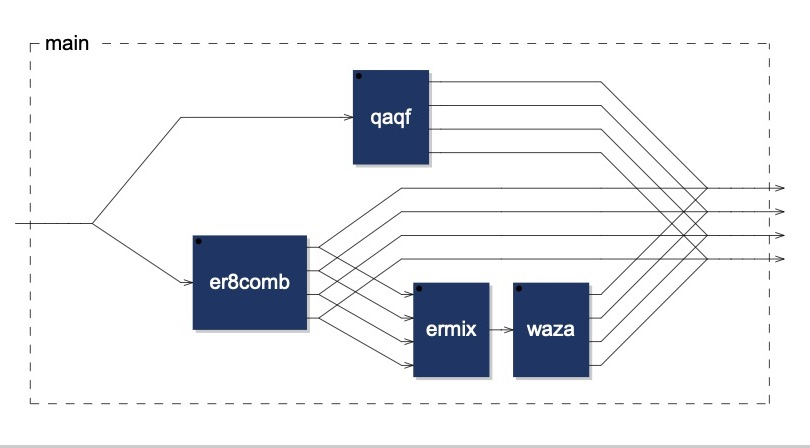
\includegraphics[width=1.\linewidth]{main}
\end{center}

\section*{\color{cbordeaux}RE-WRITING \\ THE WORDS-HOLE}

The second topology of music score has a deep electroacoustic documentation and an accurate specific musical notation. Nevertheless, the documentation requires a musicological approach to unveil the meaning of, what we defined, \emph{words-hole}.

\emph{\textbf{Risonanze Erranti}} is a long work of the latest Nono's composition period, with many live electronics instruments inside the ensemble, some of that was undocumented hardware, names without meaning, \emph{words-hole}. 

To avoid misunderstanding, every technological rewriting based on block-diagram must be a partial true. Each block named with an intergalactic \emph{words-hole} can lead everywhere. The sound of the \emph{Halaphon} (to cite one of the Nono's \emph{words-hole} block) not exist. The \emph{Halaphon} was a way to connect pure musical thinking with consolidated musical practice, embracing acoustical space and electronics. Before the instrument itself, the \emph{Halaphon}, was an idea of space-related music, that became a necessity, and only at the end an opportunity.

The difference between what could be instrument or not is very clear: the articulated performability through listening. If there is something that must be sustained is exactly that musical behaviour. Each of those Nono's words conducts the musician to agile and deeply performable electroacoustic musical environments. So it  passes the concept of an instrumental practice consolidated on the means and tools available. Nono himself talks about it by transversally crossing architecture, classical musical practice and technology, in executive and interpretative terms:

\vfill

\begin{quotation}
\begin{it}
\begin{flushright}
\noindent La musica non è solo composizione. Non è artigianato, non è un mestiere. La musica è pensiero
\end{flushright}
\end{it}
\flushright{Luigi Nono}
\end{quotation}

\columnbreak

% ------------------------------------ CLAUDIO

\begin{center}
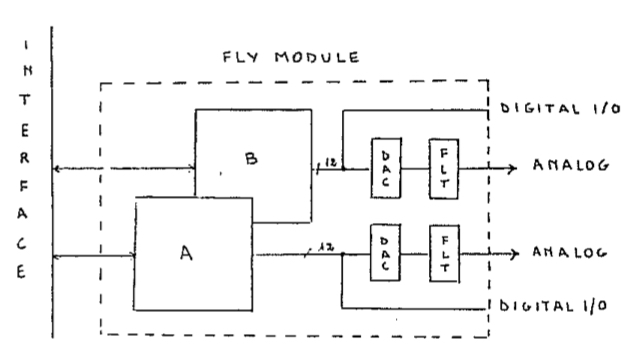
\includegraphics[width=1.\linewidth]{lmfly10}
\end{center}

\section*{\color{cbordeaux}PORTING}

The porting of aged music informatics of experimental instruments to a sustained programming language and technology merging into two branches: the history of instruments (even the technological ones) and the \emph{back to the future} of music lost in the past for technological issues, into a new possibility of music playing. 

Working side by side with Michelangelo Lupone for the \emph{\textbf{Mobile Locale}} porting is something extremely musical related and only marginally a technological and informatics matter. The main goal is the possibility to interpret his music, with his unavoidable sensibility at disposal of better comprehension of the music score. Close to this, the fascinating possibility to revive a beautiful work, \emph{Mobile Locale}, stuck by technical problems that obscured its musical value. The work was conceived around a technology born from the same Lupone's musical thinking, at Music Research Centre, in Rome, the System Fly. 

%The entire electronics, both tape and live, was conceived as a shadow of the acoustic percussions and amplification of them. So there are three levels of musical matter on stage: the acoustic (a complex set of percussions), the electroacoustic (sound reinforcement, early reflections simulation and tape), the live electronics (real-time processes based on three different delay lines usages).

%During the staging strategy, the entire sound direction must be focused on the balancing of the live electronics with the electroacoustic sound, that has to be hidden, by all of these, inside the percussion sounds.

The relationship between instrument, opera and musical idea as the core of Lupone's composition process, brings again the conversation at the necessity to have a musical instrument, not only an electronic environment, mastered to focus on expected musical behaviour. 

\vfill

\begin{quotation}
\begin{it}
\begin{flushright}
\noindent The different cultural and professional backgrounds of the members of the team (musicians, physicists, engineers and musicologists) united by a common appreciation of interdisciplinary problems and all specialising in informatic systems, produced the group's present capacity to create a digital system oriented towards the synthesis, analysis and real-time processing of sound signals. This system develops an immediate interaction with the user and it is flexible and adaptable to the different scientific and artistic needs \cite{ml91}.
\end{flushright}
\end{it}
\flushright{Michelangelo Lupone}
\end{quotation}

\columnbreak

% ------------------------------------ MICHELE

\begin{center}
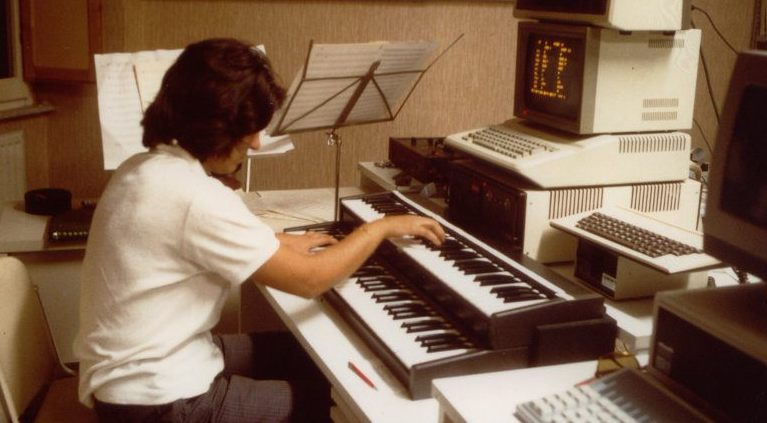
\includegraphics[width=1.\linewidth]{Fly10_Apple1}
\end{center}

\section*{\color{cbordeaux}SEAM LIBRARIES}

%Developing the concepts of the instrument and instrumentalist to the combined form of those into interpretation, requires the overcoming of obsolete parallelism: the computer music performer as an artisan of \emph{new-luthiery}. There is not a sustainability conception under the deception of that wrong and obsolete metaphor. Each \emph{luthiery} is new, it evolve with musical needs. Each instrument has his inventor and his virtuoso, but in musical history, those people never coincided. The best instruments were conceived from men entirely devoted to the conception of something unique. The best virtuoso took those instruments to unveil their prospective.

Instruments carved by musical ideas on readable text (code) becomes a sub-literature in which each brick maintain the power of the source code, the clarity of an equation, the efficiency of the continuous development, the reusability of a word in different contexts. 

Actually there are five different libraries:
\textbf{seam.lib} contains general functions and the pointers to each specific library. It may also comprehend the custom performative environment definition, as it could be for the inputs and the outputs, the setup parameters and the performative controls. \\
\textbf{gerzon.lib} contains early Michael Gerzon works, his core concepts of spatialization and stereophony, that conducted him to conceive the Ambisonic technology. In a sustained environment, the role of this library is to avoid misunderstanding of what \emph{stereo} is and what we are loosing in the electroacoustic staging perception. \\
\textbf{hardware.lib} contains hardware-related functions like MIDI mapping and I/O assignment to an audio interface, with a routing strategy to connect instruments to real-world hardware with a graphical user interface to map routing.\\
\textbf{measurement.lib} contains some audio analysis strategy to define musical display feature for audio inspection, such as integrated measurement and loudness monitoring, that are indispensable tools for today staging of public addressed music.\\
\textbf{nono.lib} is the first author-related library that points to contain \emph{Live Electronics Instruments}. The idea is to collect instruments into the library and use them, work by work, in a hardware-like approach.

\textbf{SEAM is an Open, DRY, Community.} People inside SEAM will share their knowledge to weld words, papers and literature with meaning.

\vfill

\begin{quotation}
\begin{it}
\begin{flushright}
A line where two pieces of fabric are sewn together\ldots An underground layer of a mineral such as coal or gold: the buried forests became seams of coal\ldots Join with a seam.
\end{flushright}
\end{it}
\flushright{SEAM meaning}
\end{quotation}

\end{multicols}
\end{document}